\section{Amarok::Synth\_\-STEREO\_\-XFADE\_\-skel Class Reference}
\label{classAmarok_1_1Synth__STEREO__XFADE__skel}\index{Amarok::Synth_STEREO_XFADE_skel@{Amarok::Synth\_\-STEREO\_\-XFADE\_\-skel}}
{\tt \#include $<$amarokarts.h$>$}

Inheritance diagram for Amarok::Synth\_\-STEREO\_\-XFADE\_\-skel:\begin{figure}[H]
\begin{center}
\leavevmode
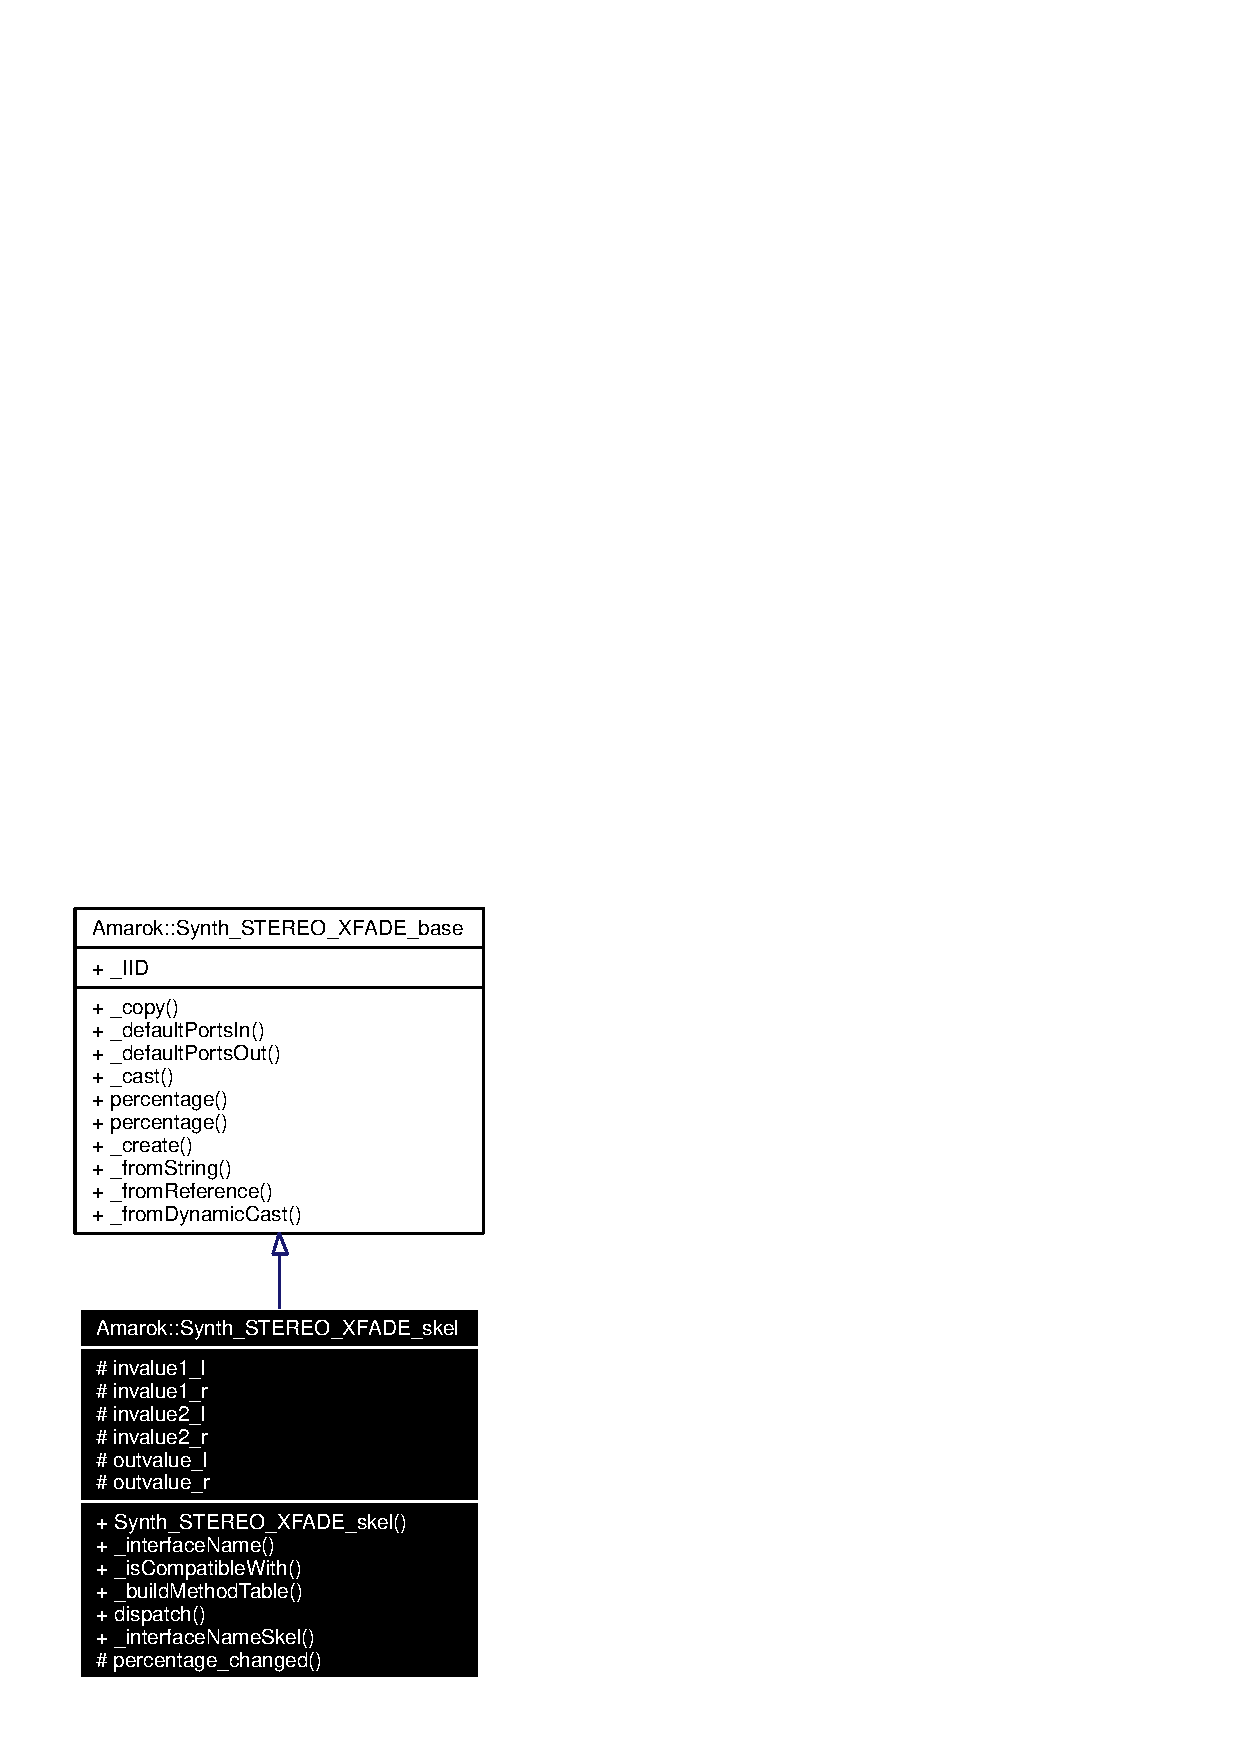
\includegraphics[width=116pt]{classAmarok_1_1Synth__STEREO__XFADE__skel__inherit__graph}
\end{center}
\end{figure}
Collaboration diagram for Amarok::Synth\_\-STEREO\_\-XFADE\_\-skel:\begin{figure}[H]
\begin{center}
\leavevmode
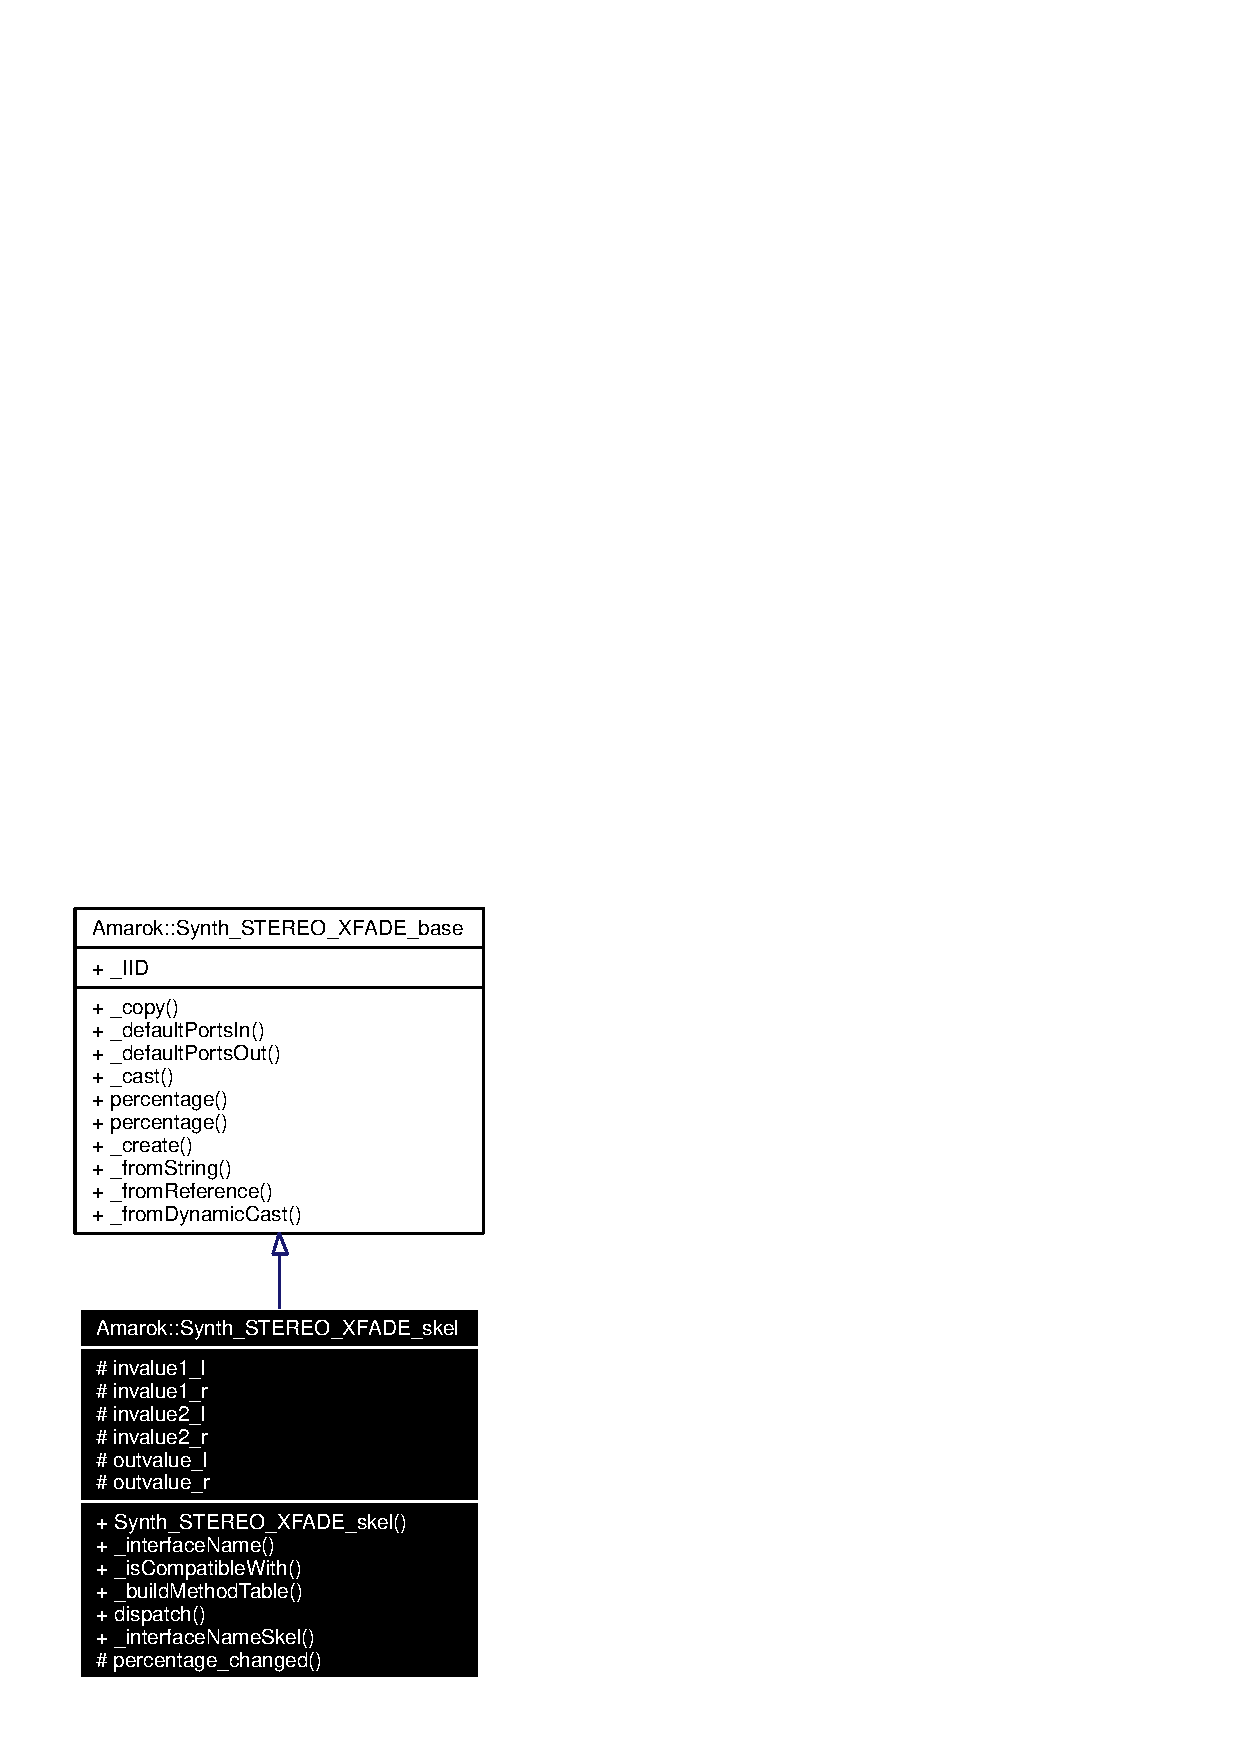
\includegraphics[width=116pt]{classAmarok_1_1Synth__STEREO__XFADE__skel__coll__graph}
\end{center}
\end{figure}
\subsection*{Public Member Functions}
\begin{CompactItemize}
\item 
{\bf Synth\_\-STEREO\_\-XFADE\_\-skel} ()
\item 
std::string {\bf \_\-interface\-Name} ()
\item 
bool {\bf \_\-is\-Compatible\-With} (const std::string \&interfacename)
\item 
void {\bf \_\-build\-Method\-Table} ()
\item 
void {\bf dispatch} (Arts::Buffer $\ast$request, Arts::Buffer $\ast$result, long method\-ID)
\item 
{\bf Synth\_\-STEREO\_\-XFADE\_\-base} $\ast$ {\bf \_\-copy} ()
\item 
virtual std::vector$<$ std::string $>$ {\bf \_\-default\-Ports\-In} () const 
\item 
virtual std::vector$<$ std::string $>$ {\bf \_\-default\-Ports\-Out} () const 
\item 
void $\ast$ {\bf \_\-cast} (unsigned long iid)
\item 
virtual float {\bf percentage} ()=0
\item 
virtual void {\bf percentage} (float new\-Value)=0
\end{CompactItemize}
\subsection*{Static Public Member Functions}
\begin{CompactItemize}
\item 
std::string {\bf \_\-interface\-Name\-Skel} ()
\item 
{\bf Synth\_\-STEREO\_\-XFADE\_\-base} $\ast$ {\bf \_\-create} (const std::string \&sub\-Class=\char`\"{}Amarok::Synth\_\-STEREO\_\-XFADE\char`\"{})
\item 
{\bf Synth\_\-STEREO\_\-XFADE\_\-base} $\ast$ {\bf \_\-from\-String} (const std::string \&objectref)
\item 
{\bf Synth\_\-STEREO\_\-XFADE\_\-base} $\ast$ {\bf \_\-from\-Reference} (Arts::Object\-Reference ref, bool needcopy)
\item 
{\bf Synth\_\-STEREO\_\-XFADE\_\-base} $\ast$ {\bf \_\-from\-Dynamic\-Cast} (const Arts::Object \&object)
\end{CompactItemize}
\subsection*{Static Public Attributes}
\begin{CompactItemize}
\item 
unsigned long {\bf \_\-IID} = Arts::MCOPUtils::make\-IID(\char`\"{}Amarok::Synth\_\-STEREO\_\-XFADE\char`\"{})
\end{CompactItemize}
\subsection*{Protected Member Functions}
\begin{CompactItemize}
\item 
void {\bf percentage\_\-changed} (float new\-Value)
\end{CompactItemize}
\subsection*{Protected Attributes}
\begin{CompactItemize}
\item 
float $\ast$ {\bf invalue1\_\-l}
\item 
float $\ast$ {\bf invalue1\_\-r}
\item 
float $\ast$ {\bf invalue2\_\-l}
\item 
float $\ast$ {\bf invalue2\_\-r}
\item 
float $\ast$ {\bf outvalue\_\-l}
\item 
float $\ast$ {\bf outvalue\_\-r}
\end{CompactItemize}


\subsection{Constructor \& Destructor Documentation}
\index{Amarok::Synth_STEREO_XFADE_skel@{Amarok::Synth\_\-STEREO\_\-XFADE\_\-skel}!Synth_STEREO_XFADE_skel@{Synth\_\-STEREO\_\-XFADE\_\-skel}}
\index{Synth_STEREO_XFADE_skel@{Synth\_\-STEREO\_\-XFADE\_\-skel}!Amarok::Synth_STEREO_XFADE_skel@{Amarok::Synth\_\-STEREO\_\-XFADE\_\-skel}}
\subsubsection{\setlength{\rightskip}{0pt plus 5cm}Amarok::Synth\_\-STEREO\_\-XFADE\_\-skel::Synth\_\-STEREO\_\-XFADE\_\-skel ()}\label{classAmarok_1_1Synth__STEREO__XFADE__skel_Amarok_1_1Synth__STEREO__XFADE__skela0}




Definition at line 166 of file amarokarts.cc.

References invalue1\_\-l, invalue1\_\-r, invalue2\_\-l, invalue2\_\-r, outvalue\_\-l, and outvalue\_\-r.



\footnotesize\begin{verbatim}167 {
168         _initStream("invalue1_l",&invalue1_l,9);
169         _initStream("invalue1_r",&invalue1_r,9);
170         _initStream("invalue2_l",&invalue2_l,9);
171         _initStream("invalue2_r",&invalue2_r,9);
172         _initStream("outvalue_l",&outvalue_l,10);
173         _initStream("outvalue_r",&outvalue_r,10);
174 }
\end{verbatim}\normalsize 


\subsection{Member Function Documentation}
\index{Amarok::Synth_STEREO_XFADE_skel@{Amarok::Synth\_\-STEREO\_\-XFADE\_\-skel}!_buildMethodTable@{\_\-buildMethodTable}}
\index{_buildMethodTable@{\_\-buildMethodTable}!Amarok::Synth_STEREO_XFADE_skel@{Amarok::Synth\_\-STEREO\_\-XFADE\_\-skel}}
\subsubsection{\setlength{\rightskip}{0pt plus 5cm}void Amarok::Synth\_\-STEREO\_\-XFADE\_\-skel::\_\-build\-Method\-Table ()}\label{classAmarok_1_1Synth__STEREO__XFADE__skel_Amarok_1_1Synth__STEREO__XFADE__skela3}




Definition at line 151 of file amarokarts.cc.

References \_\-dispatch\_\-Amarok\_\-Synth\_\-STEREO\_\-XFADE\_\-00(), and \_\-dispatch\_\-Amarok\_\-Synth\_\-STEREO\_\-XFADE\_\-01().



\footnotesize\begin{verbatim}152 {
153         Arts::Buffer m;
154         m.fromString(
155         "MethodTable:000000105f6765745f70657263656e746167650000000006666c6f"
156         "617400000000020000000000000000000000105f7365745f70657263656e746167"
157         "650000000005766f696400000000020000000100000006666c6f61740000000009"
158         "6e657756616c7565000000000000000000",
159                 "MethodTable"
160         );
161         _addMethod(_dispatch_Amarok_Synth_STEREO_XFADE_00,this,Arts::MethodDef(m));
162         _addMethod(_dispatch_Amarok_Synth_STEREO_XFADE_01,this,Arts::MethodDef(m));
163         Arts::SynthModule_skel::_buildMethodTable();
164 }
\end{verbatim}\normalsize 


Here is the call graph for this function:\begin{figure}[H]
\begin{center}
\leavevmode
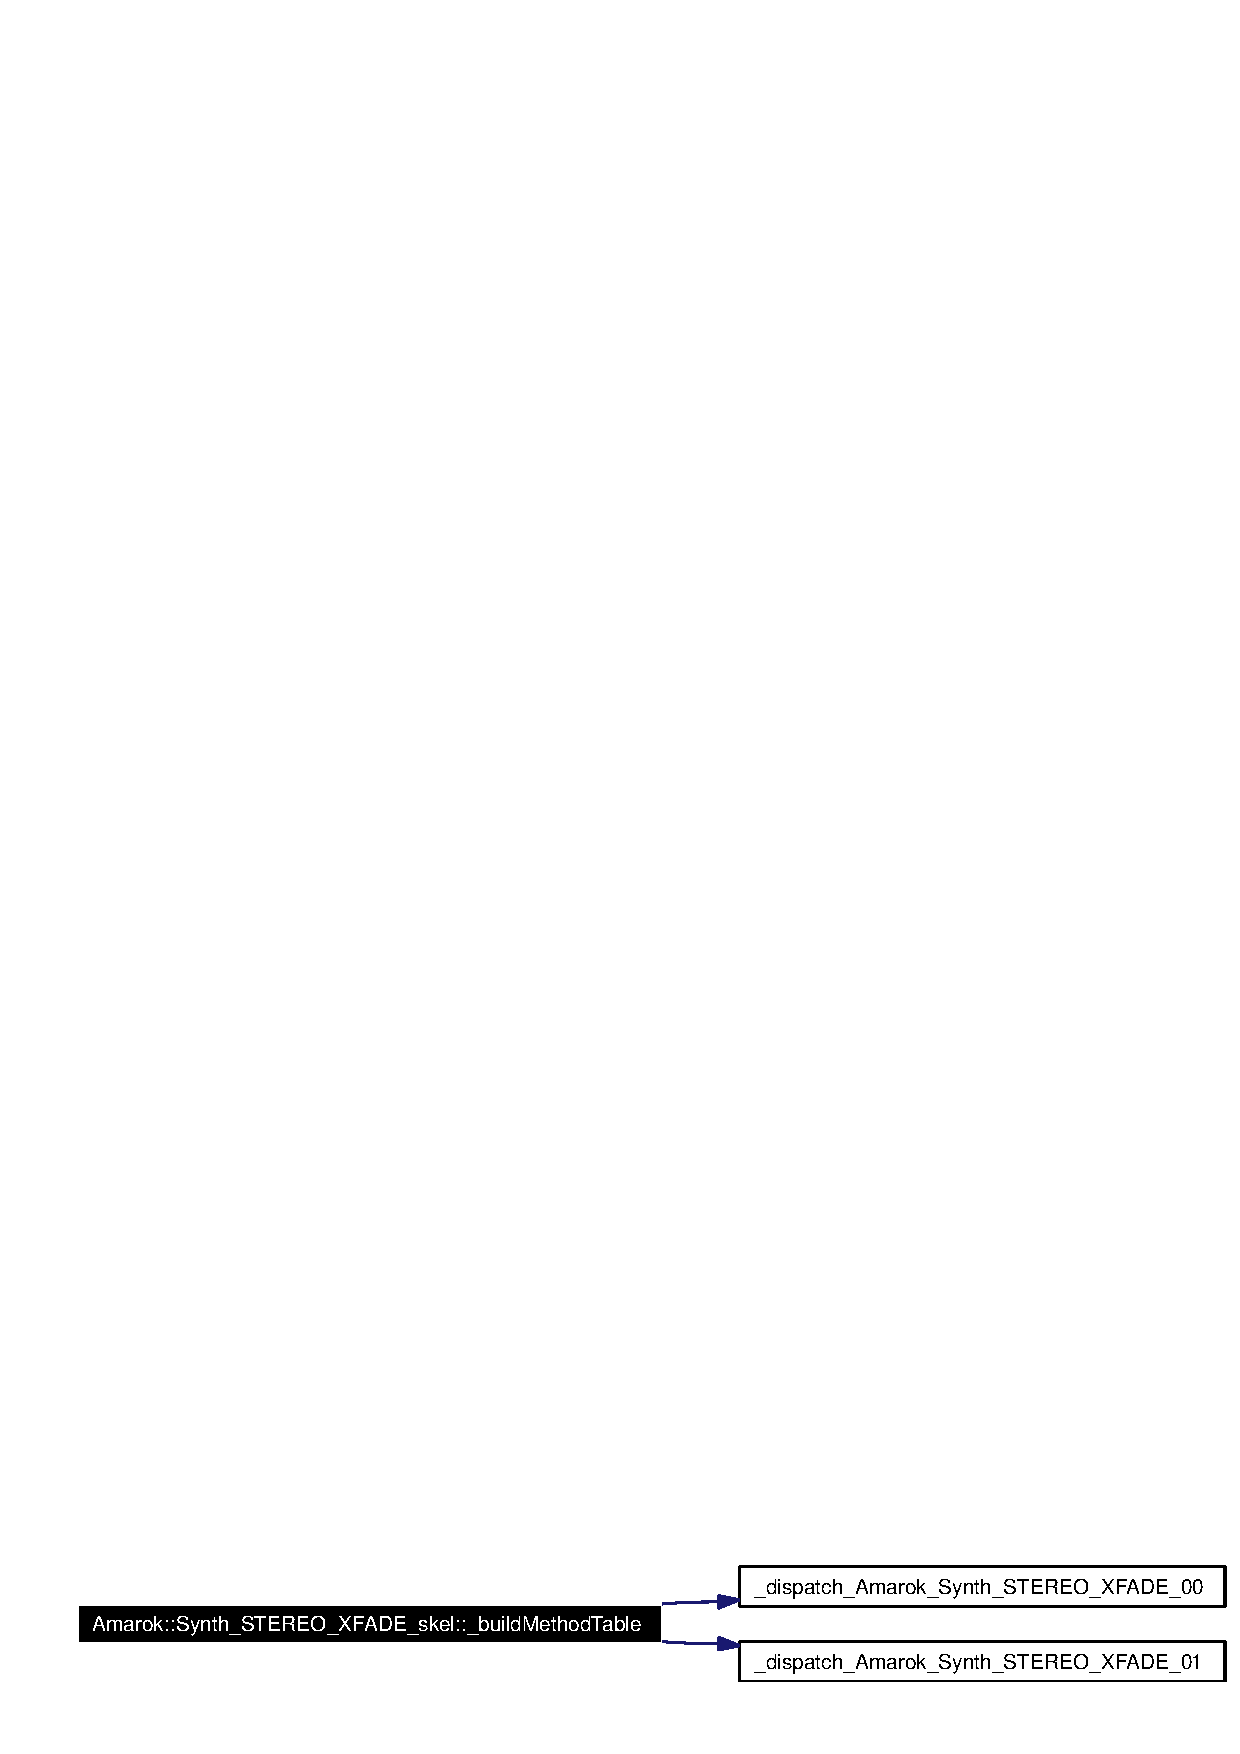
\includegraphics[width=294pt]{classAmarok_1_1Synth__STEREO__XFADE__skel_Amarok_1_1Synth__STEREO__XFADE__skela3_cgraph}
\end{center}
\end{figure}
\index{Amarok::Synth_STEREO_XFADE_skel@{Amarok::Synth\_\-STEREO\_\-XFADE\_\-skel}!_cast@{\_\-cast}}
\index{_cast@{\_\-cast}!Amarok::Synth_STEREO_XFADE_skel@{Amarok::Synth\_\-STEREO\_\-XFADE\_\-skel}}
\subsubsection{\setlength{\rightskip}{0pt plus 5cm}void $\ast$ Amarok::Synth\_\-STEREO\_\-XFADE\_\-base::\_\-cast (unsigned long {\em iid})\hspace{0.3cm}{\tt  [inherited]}}\label{classAmarok_1_1Synth__STEREO__XFADE__base_Amarok_1_1Synth__STEREO__XFADE__stuba6}




Definition at line 71 of file amarokarts.cc.

References Amarok::Synth\_\-STEREO\_\-XFADE\_\-base::\_\-IID.

Referenced by Amarok::Synth\_\-STEREO\_\-XFADE\_\-base::\_\-from\-Dynamic\-Cast(), and Amarok::Synth\_\-STEREO\_\-XFADE::\_\-method\_\-call().



\footnotesize\begin{verbatim}72 {
73         if(iid == Amarok::Synth_STEREO_XFADE_base::_IID) return (Amarok::Synth_STEREO_XFADE_base *)this;
74         if(iid == Arts::SynthModule_base::_IID) return (Arts::SynthModule_base *)this;
75         if(iid == Arts::Object_base::_IID) return (Arts::Object_base *)this;
76         return 0;
77 }
\end{verbatim}\normalsize 
\index{Amarok::Synth_STEREO_XFADE_skel@{Amarok::Synth\_\-STEREO\_\-XFADE\_\-skel}!_copy@{\_\-copy}}
\index{_copy@{\_\-copy}!Amarok::Synth_STEREO_XFADE_skel@{Amarok::Synth\_\-STEREO\_\-XFADE\_\-skel}}
\subsubsection{\setlength{\rightskip}{0pt plus 5cm}{\bf Synth\_\-STEREO\_\-XFADE\_\-base}$\ast$ Amarok::Synth\_\-STEREO\_\-XFADE\_\-base::\_\-copy ()\hspace{0.3cm}{\tt  [inline, inherited]}}\label{classAmarok_1_1Synth__STEREO__XFADE__base_Amarok_1_1Synth__STEREO__XFADE__stuba3}




Definition at line 24 of file amarokarts.h.

Referenced by Amarok::Synth\_\-STEREO\_\-XFADE\_\-base::\_\-from\-Dynamic\-Cast().



\footnotesize\begin{verbatim}24                                                 {
25                 assert(_refCnt > 0);
26                 _refCnt++;
27                 return this;
28         }
\end{verbatim}\normalsize 
\index{Amarok::Synth_STEREO_XFADE_skel@{Amarok::Synth\_\-STEREO\_\-XFADE\_\-skel}!_create@{\_\-create}}
\index{_create@{\_\-create}!Amarok::Synth_STEREO_XFADE_skel@{Amarok::Synth\_\-STEREO\_\-XFADE\_\-skel}}
\subsubsection{\setlength{\rightskip}{0pt plus 5cm}{\bf Amarok::Synth\_\-STEREO\_\-XFADE\_\-base} $\ast$ Amarok::Synth\_\-STEREO\_\-XFADE\_\-base::\_\-create (const std::string \& {\em sub\-Class} = \char`\"{}Amarok::Synth\_\-STEREO\_\-XFADE\char`\"{})\hspace{0.3cm}{\tt  [static, inherited]}}\label{classAmarok_1_1Synth__STEREO__XFADE__base_Amarok_1_1Synth__STEREO__XFADE__stube0}




Definition at line 8 of file amarokarts.cc.

References Amarok::Synth\_\-STEREO\_\-XFADE\_\-base::\_\-IID.

Referenced by Amarok::Synth\_\-STEREO\_\-XFADE::\_\-Creator().



\footnotesize\begin{verbatim}9 {
10         Arts::Object_skel *skel = Arts::ObjectManager::the()->create(subClass);
11         assert(skel);
12         Amarok::Synth_STEREO_XFADE_base *castedObject = (Amarok::Synth_STEREO_XFADE_base *)skel->_cast(Amarok::Synth_STEREO_XFADE_base::_IID);
13         assert(castedObject);
14         return castedObject;
15 }
\end{verbatim}\normalsize 
\index{Amarok::Synth_STEREO_XFADE_skel@{Amarok::Synth\_\-STEREO\_\-XFADE\_\-skel}!_defaultPortsIn@{\_\-defaultPortsIn}}
\index{_defaultPortsIn@{\_\-defaultPortsIn}!Amarok::Synth_STEREO_XFADE_skel@{Amarok::Synth\_\-STEREO\_\-XFADE\_\-skel}}
\subsubsection{\setlength{\rightskip}{0pt plus 5cm}std::vector$<$ std::string $>$ Amarok::Synth\_\-STEREO\_\-XFADE\_\-base::\_\-default\-Ports\-In () const\hspace{0.3cm}{\tt  [virtual, inherited]}}\label{classAmarok_1_1Synth__STEREO__XFADE__base_Amarok_1_1Synth__STEREO__XFADE__stuba4}




Definition at line 62 of file amarokarts.cc.



\footnotesize\begin{verbatim}62                                                                           {
63         std::vector<std::string> ret;
64         return ret;
65 }
\end{verbatim}\normalsize 
\index{Amarok::Synth_STEREO_XFADE_skel@{Amarok::Synth\_\-STEREO\_\-XFADE\_\-skel}!_defaultPortsOut@{\_\-defaultPortsOut}}
\index{_defaultPortsOut@{\_\-defaultPortsOut}!Amarok::Synth_STEREO_XFADE_skel@{Amarok::Synth\_\-STEREO\_\-XFADE\_\-skel}}
\subsubsection{\setlength{\rightskip}{0pt plus 5cm}std::vector$<$ std::string $>$ Amarok::Synth\_\-STEREO\_\-XFADE\_\-base::\_\-default\-Ports\-Out () const\hspace{0.3cm}{\tt  [virtual, inherited]}}\label{classAmarok_1_1Synth__STEREO__XFADE__base_Amarok_1_1Synth__STEREO__XFADE__stuba5}




Definition at line 66 of file amarokarts.cc.



\footnotesize\begin{verbatim}66                                                                            {
67         std::vector<std::string> ret;
68         return ret;
69 }
\end{verbatim}\normalsize 
\index{Amarok::Synth_STEREO_XFADE_skel@{Amarok::Synth\_\-STEREO\_\-XFADE\_\-skel}!_fromDynamicCast@{\_\-fromDynamicCast}}
\index{_fromDynamicCast@{\_\-fromDynamicCast}!Amarok::Synth_STEREO_XFADE_skel@{Amarok::Synth\_\-STEREO\_\-XFADE\_\-skel}}
\subsubsection{\setlength{\rightskip}{0pt plus 5cm}{\bf Amarok::Synth\_\-STEREO\_\-XFADE\_\-base} $\ast$ Amarok::Synth\_\-STEREO\_\-XFADE\_\-base::\_\-from\-Dynamic\-Cast (const Arts::Object \& {\em object})\hspace{0.3cm}{\tt  [static, inherited]}}\label{classAmarok_1_1Synth__STEREO__XFADE__base_Amarok_1_1Synth__STEREO__XFADE__stube3}




Definition at line 26 of file amarokarts.cc.

References Amarok::Synth\_\-STEREO\_\-XFADE\_\-base::\_\-cast(), Amarok::Synth\_\-STEREO\_\-XFADE\_\-base::\_\-copy(), Amarok::Synth\_\-STEREO\_\-XFADE\_\-base::\_\-from\-String(), and Amarok::Synth\_\-STEREO\_\-XFADE\_\-base::\_\-IID.



\footnotesize\begin{verbatim}27 {
28         if(object.isNull()) return 0;
29 
30         Amarok::Synth_STEREO_XFADE_base *castedObject = (Amarok::Synth_STEREO_XFADE_base *)object._base()->_cast(Amarok::Synth_STEREO_XFADE_base::_IID);
31         if(castedObject) return castedObject->_copy();
32 
33         return _fromString(object._toString());
34 }
\end{verbatim}\normalsize 


Here is the call graph for this function:\begin{figure}[H]
\begin{center}
\leavevmode
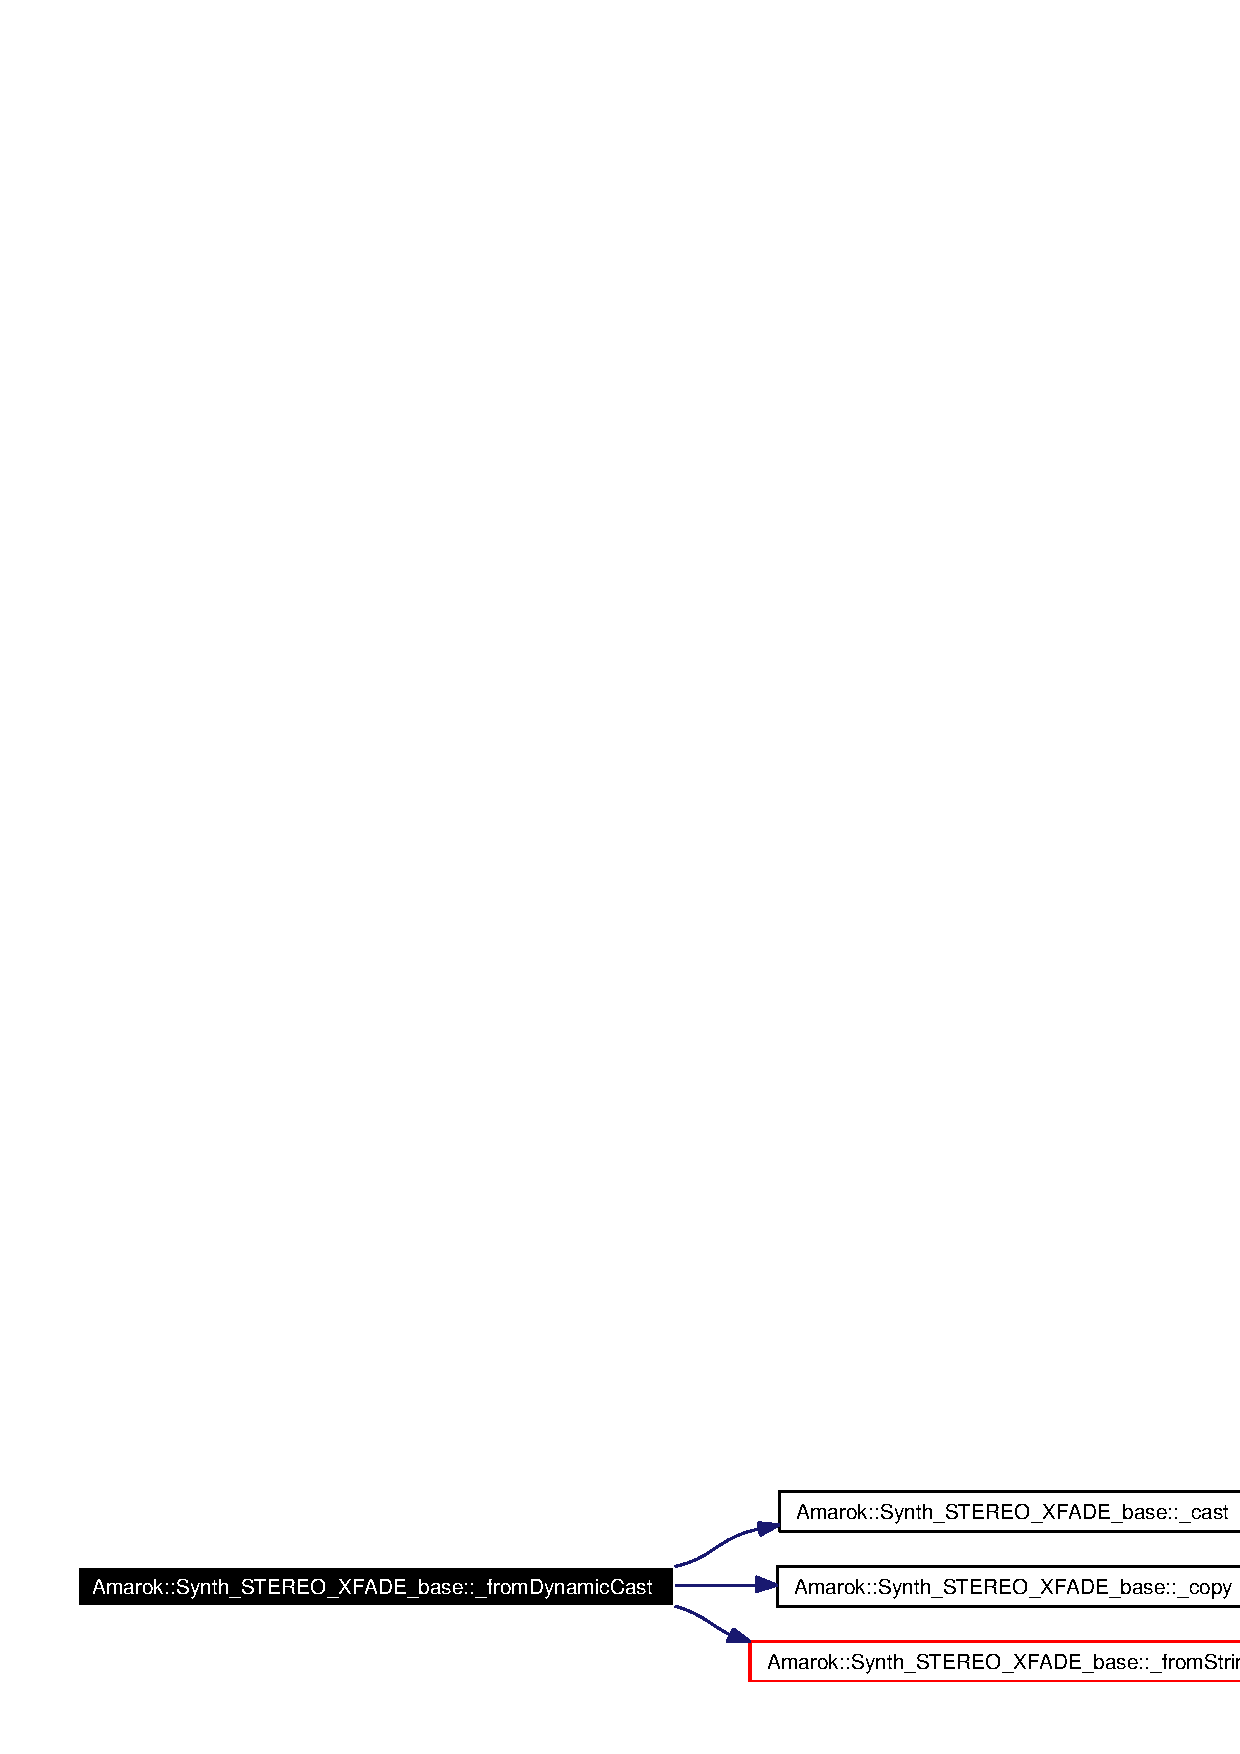
\includegraphics[width=307pt]{classAmarok_1_1Synth__STEREO__XFADE__base_Amarok_1_1Synth__STEREO__XFADE__stube3_cgraph}
\end{center}
\end{figure}
\index{Amarok::Synth_STEREO_XFADE_skel@{Amarok::Synth\_\-STEREO\_\-XFADE\_\-skel}!_fromReference@{\_\-fromReference}}
\index{_fromReference@{\_\-fromReference}!Amarok::Synth_STEREO_XFADE_skel@{Amarok::Synth\_\-STEREO\_\-XFADE\_\-skel}}
\subsubsection{\setlength{\rightskip}{0pt plus 5cm}{\bf Amarok::Synth\_\-STEREO\_\-XFADE\_\-base} $\ast$ Amarok::Synth\_\-STEREO\_\-XFADE\_\-base::\_\-from\-Reference (Arts::Object\-Reference {\em ref}, bool {\em needcopy})\hspace{0.3cm}{\tt  [static, inherited]}}\label{classAmarok_1_1Synth__STEREO__XFADE__base_Amarok_1_1Synth__STEREO__XFADE__stube2}




Definition at line 36 of file amarokarts.cc.

Referenced by Amarok::Synth\_\-STEREO\_\-XFADE\_\-base::\_\-from\-String().



\footnotesize\begin{verbatim}37 {
38         Amarok::Synth_STEREO_XFADE_base *result;
39         result = (Amarok::Synth_STEREO_XFADE_base *)Arts::Dispatcher::the()->connectObjectLocal(r,"Amarok::Synth_STEREO_XFADE");
40         if(result)
41         {
42                 if(!needcopy)
43                         result->_cancelCopyRemote();
44         }
45         else
46         {
47                 Arts::Connection *conn = Arts::Dispatcher::the()->connectObjectRemote(r);
48                 if(conn)
49                 {
50                         result = new Amarok::Synth_STEREO_XFADE_stub(conn,r.objectID);
51                         if(needcopy) result->_copyRemote();
52                         result->_useRemote();
53                         if (!result->_isCompatibleWith("Amarok::Synth_STEREO_XFADE")) {
54                                 result->_release();
55                                 return 0;
56                         }
57                 }
58         }
59         return result;
60 }
\end{verbatim}\normalsize 
\index{Amarok::Synth_STEREO_XFADE_skel@{Amarok::Synth\_\-STEREO\_\-XFADE\_\-skel}!_fromString@{\_\-fromString}}
\index{_fromString@{\_\-fromString}!Amarok::Synth_STEREO_XFADE_skel@{Amarok::Synth\_\-STEREO\_\-XFADE\_\-skel}}
\subsubsection{\setlength{\rightskip}{0pt plus 5cm}{\bf Amarok::Synth\_\-STEREO\_\-XFADE\_\-base} $\ast$ Amarok::Synth\_\-STEREO\_\-XFADE\_\-base::\_\-from\-String (const std::string \& {\em objectref})\hspace{0.3cm}{\tt  [static, inherited]}}\label{classAmarok_1_1Synth__STEREO__XFADE__base_Amarok_1_1Synth__STEREO__XFADE__stube1}




Definition at line 17 of file amarokarts.cc.

References Amarok::Synth\_\-STEREO\_\-XFADE\_\-base::\_\-from\-Reference().

Referenced by Amarok::Synth\_\-STEREO\_\-XFADE\_\-base::\_\-from\-Dynamic\-Cast().



\footnotesize\begin{verbatim}18 {
19         Arts::ObjectReference r;
20 
21         if(Arts::Dispatcher::the()->stringToObjectReference(r,objectref))
22                 return Amarok::Synth_STEREO_XFADE_base::_fromReference(r,true);
23         return 0;
24 }
\end{verbatim}\normalsize 


Here is the call graph for this function:\begin{figure}[H]
\begin{center}
\leavevmode
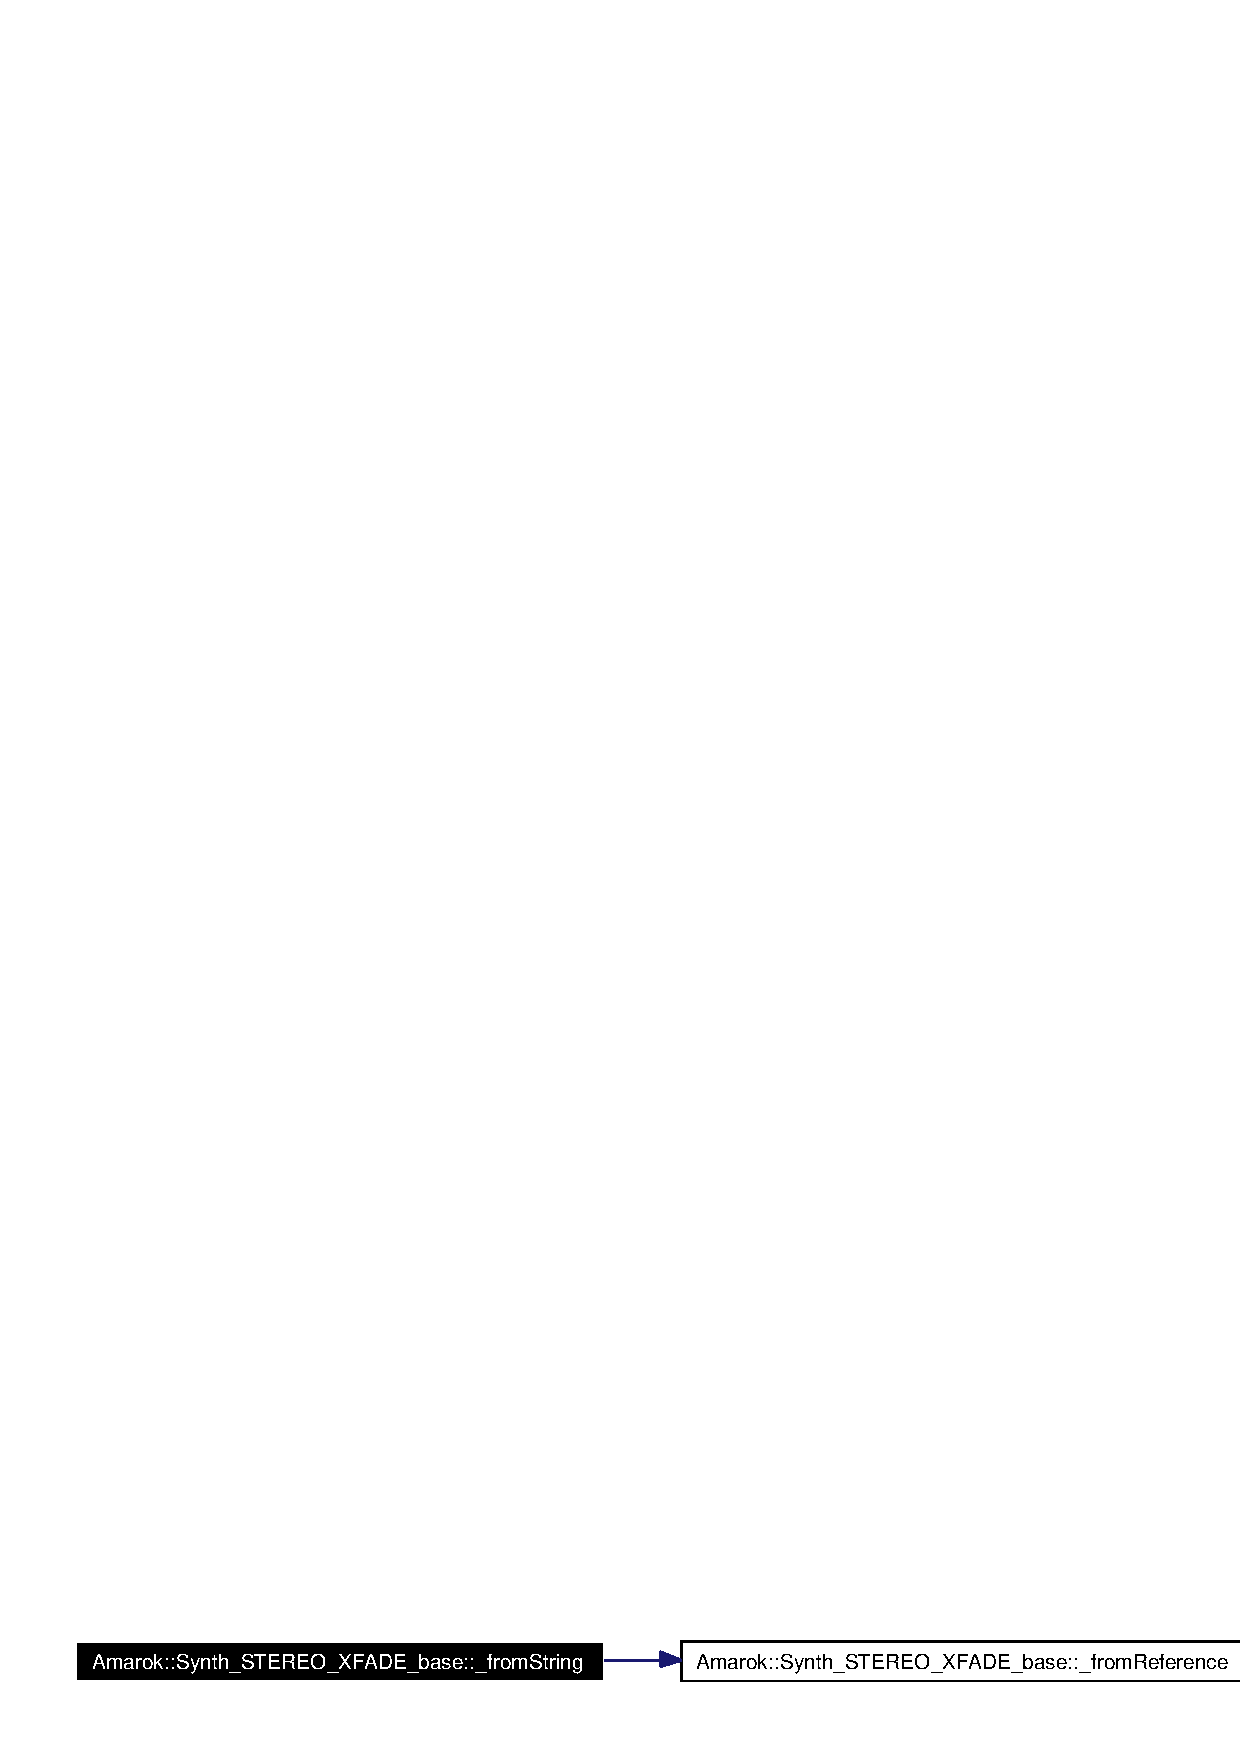
\includegraphics[width=300pt]{classAmarok_1_1Synth__STEREO__XFADE__base_Amarok_1_1Synth__STEREO__XFADE__stube1_cgraph}
\end{center}
\end{figure}
\index{Amarok::Synth_STEREO_XFADE_skel@{Amarok::Synth\_\-STEREO\_\-XFADE\_\-skel}!_interfaceName@{\_\-interfaceName}}
\index{_interfaceName@{\_\-interfaceName}!Amarok::Synth_STEREO_XFADE_skel@{Amarok::Synth\_\-STEREO\_\-XFADE\_\-skel}}
\subsubsection{\setlength{\rightskip}{0pt plus 5cm}std::string Amarok::Synth\_\-STEREO\_\-XFADE\_\-skel::\_\-interface\-Name ()}\label{classAmarok_1_1Synth__STEREO__XFADE__skel_Amarok_1_1Synth__STEREO__XFADE__skela1}




Definition at line 120 of file amarokarts.cc.



\footnotesize\begin{verbatim}121 {
122         return "Amarok::Synth_STEREO_XFADE";
123 }
\end{verbatim}\normalsize 
\index{Amarok::Synth_STEREO_XFADE_skel@{Amarok::Synth\_\-STEREO\_\-XFADE\_\-skel}!_interfaceNameSkel@{\_\-interfaceNameSkel}}
\index{_interfaceNameSkel@{\_\-interfaceNameSkel}!Amarok::Synth_STEREO_XFADE_skel@{Amarok::Synth\_\-STEREO\_\-XFADE\_\-skel}}
\subsubsection{\setlength{\rightskip}{0pt plus 5cm}std::string Amarok::Synth\_\-STEREO\_\-XFADE\_\-skel::\_\-interface\-Name\-Skel ()\hspace{0.3cm}{\tt  [static]}}\label{classAmarok_1_1Synth__STEREO__XFADE__skel_Amarok_1_1Synth__STEREO__XFADE__skele0}




Definition at line 133 of file amarokarts.cc.



\footnotesize\begin{verbatim}134 {
135         return "Amarok::Synth_STEREO_XFADE";
136 }
\end{verbatim}\normalsize 
\index{Amarok::Synth_STEREO_XFADE_skel@{Amarok::Synth\_\-STEREO\_\-XFADE\_\-skel}!_isCompatibleWith@{\_\-isCompatibleWith}}
\index{_isCompatibleWith@{\_\-isCompatibleWith}!Amarok::Synth_STEREO_XFADE_skel@{Amarok::Synth\_\-STEREO\_\-XFADE\_\-skel}}
\subsubsection{\setlength{\rightskip}{0pt plus 5cm}bool Amarok::Synth\_\-STEREO\_\-XFADE\_\-skel::\_\-is\-Compatible\-With (const std::string \& {\em interfacename})}\label{classAmarok_1_1Synth__STEREO__XFADE__skel_Amarok_1_1Synth__STEREO__XFADE__skela2}




Definition at line 125 of file amarokarts.cc.



\footnotesize\begin{verbatim}126 {
127         if (interfacename == "Amarok::Synth_STEREO_XFADE") return true;
128         if (interfacename == "Arts::SynthModule") return true;
129         if (interfacename == "Arts::Object") return true;
130         return false;
131 }
\end{verbatim}\normalsize 
\index{Amarok::Synth_STEREO_XFADE_skel@{Amarok::Synth\_\-STEREO\_\-XFADE\_\-skel}!dispatch@{dispatch}}
\index{dispatch@{dispatch}!Amarok::Synth_STEREO_XFADE_skel@{Amarok::Synth\_\-STEREO\_\-XFADE\_\-skel}}
\subsubsection{\setlength{\rightskip}{0pt plus 5cm}void Amarok::Synth\_\-STEREO\_\-XFADE\_\-skel::dispatch (Arts::Buffer $\ast$ {\em request}, Arts::Buffer $\ast$ {\em result}, long {\em method\-ID})}\label{classAmarok_1_1Synth__STEREO__XFADE__skel_Amarok_1_1Synth__STEREO__XFADE__skela4}


\index{Amarok::Synth_STEREO_XFADE_skel@{Amarok::Synth\_\-STEREO\_\-XFADE\_\-skel}!percentage@{percentage}}
\index{percentage@{percentage}!Amarok::Synth_STEREO_XFADE_skel@{Amarok::Synth\_\-STEREO\_\-XFADE\_\-skel}}
\subsubsection{\setlength{\rightskip}{0pt plus 5cm}virtual void Amarok::Synth\_\-STEREO\_\-XFADE\_\-base::percentage (float {\em new\-Value})\hspace{0.3cm}{\tt  [pure virtual, inherited]}}\label{classAmarok_1_1Synth__STEREO__XFADE__base_Amarok_1_1Synth__STEREO__XFADE__skela10}




Implemented in {\bf Amarok::Synth\_\-STEREO\_\-XFADE\_\-stub} {\rm (p.\,\pageref{classAmarok_1_1Synth__STEREO__XFADE__stub_Amarok_1_1Synth__STEREO__XFADE__stuba2})}.\index{Amarok::Synth_STEREO_XFADE_skel@{Amarok::Synth\_\-STEREO\_\-XFADE\_\-skel}!percentage@{percentage}}
\index{percentage@{percentage}!Amarok::Synth_STEREO_XFADE_skel@{Amarok::Synth\_\-STEREO\_\-XFADE\_\-skel}}
\subsubsection{\setlength{\rightskip}{0pt plus 5cm}virtual float Amarok::Synth\_\-STEREO\_\-XFADE\_\-base::percentage ()\hspace{0.3cm}{\tt  [pure virtual, inherited]}}\label{classAmarok_1_1Synth__STEREO__XFADE__base_Amarok_1_1Synth__STEREO__XFADE__skela9}




Implemented in {\bf Amarok::Synth\_\-STEREO\_\-XFADE\_\-stub} {\rm (p.\,\pageref{classAmarok_1_1Synth__STEREO__XFADE__stub_Amarok_1_1Synth__STEREO__XFADE__stuba1})}.

Referenced by Amarok::Synth\_\-STEREO\_\-XFADE::percentage().\index{Amarok::Synth_STEREO_XFADE_skel@{Amarok::Synth\_\-STEREO\_\-XFADE\_\-skel}!percentage_changed@{percentage\_\-changed}}
\index{percentage_changed@{percentage\_\-changed}!Amarok::Synth_STEREO_XFADE_skel@{Amarok::Synth\_\-STEREO\_\-XFADE\_\-skel}}
\subsubsection{\setlength{\rightskip}{0pt plus 5cm}void Amarok::Synth\_\-STEREO\_\-XFADE\_\-skel::percentage\_\-changed (float {\em new\-Value})\hspace{0.3cm}{\tt  [inline, protected]}}\label{classAmarok_1_1Synth__STEREO__XFADE__skel_Amarok_1_1Synth__STEREO__XFADE__skelb0}




Definition at line 62 of file amarokarts.h.



\footnotesize\begin{verbatim}62                                                        {
63                 _emit_changed("percentage_changed",newValue);
64         }
\end{verbatim}\normalsize 


\subsection{Member Data Documentation}
\index{Amarok::Synth_STEREO_XFADE_skel@{Amarok::Synth\_\-STEREO\_\-XFADE\_\-skel}!_IID@{\_\-IID}}
\index{_IID@{\_\-IID}!Amarok::Synth_STEREO_XFADE_skel@{Amarok::Synth\_\-STEREO\_\-XFADE\_\-skel}}
\subsubsection{\setlength{\rightskip}{0pt plus 5cm}unsigned long {\bf Amarok::Synth\_\-STEREO\_\-XFADE\_\-base::\_\-IID} = Arts::MCOPUtils::make\-IID(\char`\"{}Amarok::Synth\_\-STEREO\_\-XFADE\char`\"{})\hspace{0.3cm}{\tt  [static, inherited]}}\label{classAmarok_1_1Synth__STEREO__XFADE__base_Amarok_1_1Synth__STEREO__XFADE__stubs0}




Definition at line 180 of file amarokarts.cc.

Referenced by Amarok::Synth\_\-STEREO\_\-XFADE\_\-base::\_\-cast(), Amarok::Synth\_\-STEREO\_\-XFADE\_\-base::\_\-create(), and Amarok::Synth\_\-STEREO\_\-XFADE\_\-base::\_\-from\-Dynamic\-Cast().\index{Amarok::Synth_STEREO_XFADE_skel@{Amarok::Synth\_\-STEREO\_\-XFADE\_\-skel}!invalue1_l@{invalue1\_\-l}}
\index{invalue1_l@{invalue1\_\-l}!Amarok::Synth_STEREO_XFADE_skel@{Amarok::Synth\_\-STEREO\_\-XFADE\_\-skel}}
\subsubsection{\setlength{\rightskip}{0pt plus 5cm}float$\ast$ {\bf Amarok::Synth\_\-STEREO\_\-XFADE\_\-skel::invalue1\_\-l}\hspace{0.3cm}{\tt  [protected]}}\label{classAmarok_1_1Synth__STEREO__XFADE__skel_Amarok_1_1Synth__STEREO__XFADE__skelp0}




Definition at line 53 of file amarokarts.h.

Referenced by Synth\_\-STEREO\_\-XFADE\_\-skel().\index{Amarok::Synth_STEREO_XFADE_skel@{Amarok::Synth\_\-STEREO\_\-XFADE\_\-skel}!invalue1_r@{invalue1\_\-r}}
\index{invalue1_r@{invalue1\_\-r}!Amarok::Synth_STEREO_XFADE_skel@{Amarok::Synth\_\-STEREO\_\-XFADE\_\-skel}}
\subsubsection{\setlength{\rightskip}{0pt plus 5cm}float$\ast$ {\bf Amarok::Synth\_\-STEREO\_\-XFADE\_\-skel::invalue1\_\-r}\hspace{0.3cm}{\tt  [protected]}}\label{classAmarok_1_1Synth__STEREO__XFADE__skel_Amarok_1_1Synth__STEREO__XFADE__skelp1}




Definition at line 54 of file amarokarts.h.

Referenced by Synth\_\-STEREO\_\-XFADE\_\-skel().\index{Amarok::Synth_STEREO_XFADE_skel@{Amarok::Synth\_\-STEREO\_\-XFADE\_\-skel}!invalue2_l@{invalue2\_\-l}}
\index{invalue2_l@{invalue2\_\-l}!Amarok::Synth_STEREO_XFADE_skel@{Amarok::Synth\_\-STEREO\_\-XFADE\_\-skel}}
\subsubsection{\setlength{\rightskip}{0pt plus 5cm}float$\ast$ {\bf Amarok::Synth\_\-STEREO\_\-XFADE\_\-skel::invalue2\_\-l}\hspace{0.3cm}{\tt  [protected]}}\label{classAmarok_1_1Synth__STEREO__XFADE__skel_Amarok_1_1Synth__STEREO__XFADE__skelp2}




Definition at line 55 of file amarokarts.h.

Referenced by Synth\_\-STEREO\_\-XFADE\_\-skel().\index{Amarok::Synth_STEREO_XFADE_skel@{Amarok::Synth\_\-STEREO\_\-XFADE\_\-skel}!invalue2_r@{invalue2\_\-r}}
\index{invalue2_r@{invalue2\_\-r}!Amarok::Synth_STEREO_XFADE_skel@{Amarok::Synth\_\-STEREO\_\-XFADE\_\-skel}}
\subsubsection{\setlength{\rightskip}{0pt plus 5cm}float$\ast$ {\bf Amarok::Synth\_\-STEREO\_\-XFADE\_\-skel::invalue2\_\-r}\hspace{0.3cm}{\tt  [protected]}}\label{classAmarok_1_1Synth__STEREO__XFADE__skel_Amarok_1_1Synth__STEREO__XFADE__skelp3}




Definition at line 56 of file amarokarts.h.

Referenced by Synth\_\-STEREO\_\-XFADE\_\-skel().\index{Amarok::Synth_STEREO_XFADE_skel@{Amarok::Synth\_\-STEREO\_\-XFADE\_\-skel}!outvalue_l@{outvalue\_\-l}}
\index{outvalue_l@{outvalue\_\-l}!Amarok::Synth_STEREO_XFADE_skel@{Amarok::Synth\_\-STEREO\_\-XFADE\_\-skel}}
\subsubsection{\setlength{\rightskip}{0pt plus 5cm}float$\ast$ {\bf Amarok::Synth\_\-STEREO\_\-XFADE\_\-skel::outvalue\_\-l}\hspace{0.3cm}{\tt  [protected]}}\label{classAmarok_1_1Synth__STEREO__XFADE__skel_Amarok_1_1Synth__STEREO__XFADE__skelp4}




Definition at line 57 of file amarokarts.h.

Referenced by Synth\_\-STEREO\_\-XFADE\_\-skel().\index{Amarok::Synth_STEREO_XFADE_skel@{Amarok::Synth\_\-STEREO\_\-XFADE\_\-skel}!outvalue_r@{outvalue\_\-r}}
\index{outvalue_r@{outvalue\_\-r}!Amarok::Synth_STEREO_XFADE_skel@{Amarok::Synth\_\-STEREO\_\-XFADE\_\-skel}}
\subsubsection{\setlength{\rightskip}{0pt plus 5cm}float$\ast$ {\bf Amarok::Synth\_\-STEREO\_\-XFADE\_\-skel::outvalue\_\-r}\hspace{0.3cm}{\tt  [protected]}}\label{classAmarok_1_1Synth__STEREO__XFADE__skel_Amarok_1_1Synth__STEREO__XFADE__skelp5}




Definition at line 58 of file amarokarts.h.

Referenced by Synth\_\-STEREO\_\-XFADE\_\-skel().

The documentation for this class was generated from the following files:\begin{CompactItemize}
\item 
{\bf amarokarts.h}\item 
{\bf amarokarts.cc}\end{CompactItemize}
